\documentclass[11pt]{beamer}
\usetheme{Warsaw}
\usepackage[utf8]{inputenc}
\usepackage[brazil]{babel}  % idioma
\usepackage{amsmath,amsfonts,amssymb,textcomp}
\usepackage{graphicx}
\usepackage{subfigure}

\usepackage[lined]{algorithm2e}

% Configurando layout para mostrar codigos C++
\usepackage{listings}
%\usepackage{minted}
%pdflatex -shell-escape minted01.tex
%ou
%latexmk -pdf -shell-escape minted01.tex

\author{Othon Oliveira}
\title{Sistemas Operacionais}
%\setbeamercovered{transparent} 
%\setbeamertemplate{navigation symbols}{} 
%\logo{} 
\institute{Fatec -- Faculdade de Informática --- PE} 
%\date{} 
%\subject{} 
\begin{document}


% Capa - requer o TikZ
\newcommand{\capa}{
    \begin{tikzpicture}[remember picture,overlay]
        \node at (current page.south west)
            {\begin{tikzpicture}[remember picture, overlay]
                \fill[shading=radial,top color=orange,bottom color=orange,middle color=yellow] (0,0) rectangle (\paperwidth,\paperheight);
            \end{tikzpicture}
          };
    \end{tikzpicture}
}




\begin{frame}
\titlepage
\end{frame}

\begin{frame}
\tableofcontents
\end{frame}

%+++++++++++++++++++++++++++++++++++++++++++++++
\begin{frame}{Monitores -- Starvation}
\begin{figure}[h]
%\left

\includegraphics[width=18mm, height=15mm]{Figuras/appleOficial.jpg}
\qquad \quad \quad \quad \quad

\includegraphics[width=19mm, height=17mm]{Figuras/windows.png}
\qquad \quad \quad \quad \quad \quad \quad 	\vspace{1.0in}

\includegraphics[width=15mm, height=15mm]{Figuras/android.jpg}
\qquad \quad \quad \quad \quad \quad \quad \quad 

\includegraphics[width=25mm, height=15mm]{Figuras/ubuntu_904.jpg}

\end{figure}
\end{frame}


%+++++++++++++++++++++++++++++++++++++++++++++++
\section{ Gerenciamento de Memória}
\subsection*{ Gestão básica}

\begin{frame}\frametitle{ Memória -- Recurso Importante}
  
\pause
\begin{alertblock} { Como usar recursos}
\begin{enumerate}
\pause
 \item Nenhum computador tem memória infinita,
\pause
 \item A memória é volátil (todas?)
\pause
 \item Memórias têm custo elevado (?)
\end{enumerate}
\end{alertblock} 
\end{frame}

%--------------------------------------------------------------
\begin{frame}\frametitle{ Hierarquia}
 \pause
 
\begin{alertblock}{ Hirarquia de memória}
 \pause
 A maioria dos computadores utiliza uma espécia de hierarquia.
 \begin{enumerate}
  \pause
  \item Uma pequena quantidade de memória cache, volátil, muito rápida e de custo elevado;
  \pause
  \item Uma grande quantidade de memória (RAM), volátil, de velocidade e custo médio;
  \pause
  \item Uma memória secundária, não volátil, com dezenas de centenas de gibabytes, com velocidade e custos baixos.
 \end{enumerate}
\pause
 Cabe aos Sistemas Operacionais coordenarem a utilização dessas memórias.

 \end{alertblock}
\end{frame}



%--------------------------------------------------------------
\begin{frame}\frametitle{ Gerenciamento básico de memória}
 \pause
 
\begin{block}{ Classes de sistemas gerenciadores}
 \pause
  Sistemas que, durante a execução, levam e trazem processos entre a memória principal e o disco: troca de processos e paginação, e
 \pause
  Sistemas mais simples, que não fazem essa tecnologia, Estudaremos os mais simples primeiro.
 \end{block}
 \pause
 O sistema de troca e paginação em suma são artifícios criados devido à insuficiência de memória principal para armazenar 
 simultaneamente todos os programas.
\end{frame}

%--------------------------------------------------------
\begin{frame}\frametitle{ Monoprogramação}

\begin{block}{ Sem troca de processos ou paginação}
\pause
  Quanto se utiliza um sistema mais simples de gerenciamento, a memória é compartilhada entre o programa e o sistema operacional.
  O sistema operacional pode estar na base (RAM) ou no topo (ROM). Qual desss exemplos é usado em sistemas embarcados?
\pause
  \begin{figure}[h]
    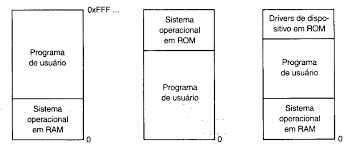
\includegraphics[width=60mm, height=30mm]{Figuras/SistemaMemSimples.png}\\
  \end{figure}
\end{block}

\end{frame}


%--------------------------------------------------------
\begin{frame}\frametitle{ Multiprogramação}

\begin{exampleblock}{ Multiplos processos a executar simultaneamente}
  A maioria dos sistemas modernos permite que múltiplos processos estejam em execução simultaneamente, o que significa que 
  quando um processo está bloqueado -- por exemplo, para esperar que uma E/S seja finalizada -- outro processo poderá usar a CPU.
\pause
  Assim a Multiprogramação aumenta a utilização da CPU. Servidores de rede sempre possuem a capacidade de execução de múltiplos 
  processos.
\end{exampleblock}

\pause
\begin{alertblock}{ Particionamento}
  A maneira mais simples de Multiprogramação é o Particionamento da Memória em n partições (de tamanhos diferentes ?)
\end{alertblock}
\end{frame}


%+++++++++++++++++++++++++++++++++++++++++++++++
\begin{frame}\frametitle{ Dois modelos de Multiprogramação}
  Partições fixas de memória separadas com filas para cada partição e com fila única de entrada.
\begin{exampleblock}{ Mutiplas filas}
  \pause
  \begin{figure}[h]
    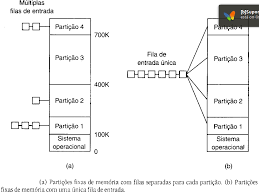
\includegraphics[width=70mm, height=40mm]{Figuras/multifilasParticap.png}\\
  \end{figure}
\end{exampleblock}
  A Multiprogramação pode melhorar a utilização da CPU.
\end{frame}


%------------------------------------------------
\begin{frame}{ Modelagem Multiprogramação}
\pause
  De modo genérico se um processo permanece em execução 20\% do tempo em memória, 
  com cinco processos em tese a CPU ficaria ocupara todo o tempo. Esse processo é otimista.
  Na realidade um modelo probabilístico. 
  Se um processo gasta \textit{p} de seu tempo, com \textit{n} processos estaria ociosa 
  \textit{$p^{n}$}.
\pause
\begin{exampleblock}{Grau de Multiprogramação}
 Utilização da CPU = 1 -- \textit{$p^{n}$}
\end{exampleblock}

 
\end{frame}




%+++++++++++++++++++++++++++++++++++++++++++++++
\section{ Troca de Processos}
\subsection*{ Gestão de memória}


\begin{frame}\frametitle{ Os métodos gerais de gerenciamento de memória}

\begin{block}{ Swapping}
 Consiste em trazer totalmente cada processo para a memória, executá-lo durante certo tempo e então devolvê-lo ao disco.
\end{block}

\pause
\begin{block}{ Memória vitual}
  A outra estratégia é denomindada \textbf{memória virtual} permite que processos sejam executados mesmo que estejam parcialmente 
  carregados na memória principal.
\end{block}

\pause
  Veremos as duas estratégias !!
\end{frame}

%----------------------------------------------------

\begin{frame}\frametitle{ Funcionamento do sistema de troca}
  A medida que os processo entram e saem a região sombreada (não utilizada) cresce ou descresce
\pause
\begin{exampleblock}{ Alocação de memória}
\pause
  \begin{figure}[h]
    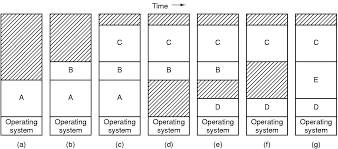
\includegraphics[width=70mm, height=40mm]{Figuras/alocacaoSemPilha.png}\\
  \end{figure}

\end{exampleblock}
  
\end{frame}

%---------------------------------------------------------------
\begin{frame}\frametitle{ Funcionamento do sistema de troca}
  Os processos crescem a medida que são execatados, provavelmente será uma boa ideia alocar memória extra (heap) sempre que se fizer 
  a tranferência de um processo para a memória ou a movimentação dele na memória!!
\pause
\begin{exampleblock}{ Alocação de memória}
\pause
  \begin{figure}[h]
    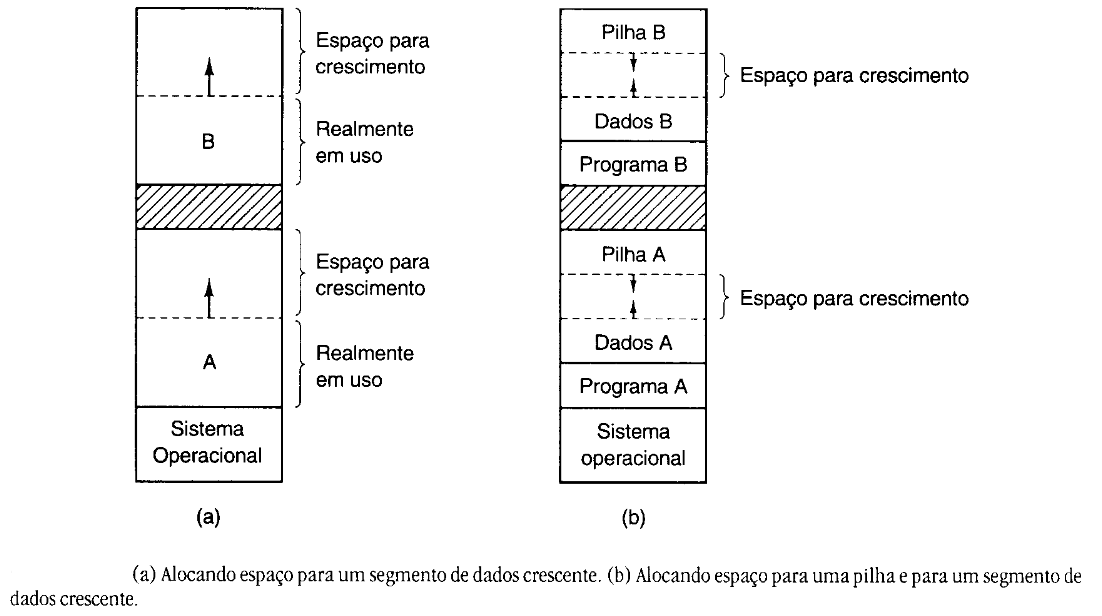
\includegraphics[width=80mm, height=40mm]{Figuras/alocacaoMemoria.png}\\
  \end{figure}

\end{exampleblock}

\end{frame}



\end{document}